
\chapter{Analyse et conception}

\section*{Introduction}
\addcontentsline{toc}{section}{Introduction}

Ce chapitre a pour objectif de définir les fondations du simulateur \textbf{ISO 8583} à travers une analyse précise des besoins ainsi que des spécifications fonctionnelles et techniques.

Il débute par une étude de l’existant dans le domaine de la monétique et du protocole \textbf{ISO 8583}, afin de justifier la pertinence du projet. Ensuite, les besoins fonctionnels et non fonctionnels sont détaillés, accompagnés d’une description des choix architecturaux retenus, notamment l’approche \textit{microservices}.

Cette étape vise à assurer une compréhension globale du système à développer, tout en posant des bases solides pour les phases ultérieures de conception et de développement.


\section{Étude fonctionnelle}
\subsection{Besoins fonctionnels}

Les besoins fonctionnels déterminent les fonctionnalités majeures attendues du système, c'est-à-dire ce que doit faire le simulateur pour répondre aux attentes des utilisateurs finaux (administrateurs et testeurs). Dans le cas du simulateur ISO 8583, ces besoins s'articulent autour de la génération, du dépaquetage et de l'analyse des messages ISO, dans un environnement sécurisé et autonome.

\begin{itemize}[label=\textbullet]
    \item \textbf{Génération de messages ISO 8583 :} Le système doit permettre à l'utilisateur de construire un message ISO à partir de 49 champs éditables, conformément au standard ISO 8583. Il doit intégrer la bibliothèque \texttt{JPos} (version 2.1.4) pour générer un message conforme au standard ISO 8583.
    
    \item \textbf{Dépaquetage de messages ISO :} Le simulateur doit être capable d'analyser et de décomposer des messages ISO bruts en champs structurés pour faciliter la compréhension et le débogage.
    
    \item \textbf{Simulation des réponses :} Le système doit simuler des réponses ISO avec différents codes de statut (\textit{succès, échec}) et codes d'erreur pour tester divers scénarios.
    
    \item \textbf{Validation syntaxique des messages :} Le simulateur doit effectuer une vérification de la syntaxe des messages avant génération, notamment la validité du MTI et la présence des champs obligatoires.
    
    \item \textbf{Affichage et journalisation des logs :} Toutes les opérations (génération, dépaquetage, réponses) doivent être tracées dans des fichiers de log. Le système doit permettre la visualisation de ces logs via l'interface de monitoring intégrée.
    
    \item \textbf{Historique des transactions :} Le système doit conserver un historique des messages ISO générés et des réponses simulées, accessible à tout moment pour consultation ou audit.
    
    \item \textbf{Gestion des utilisateurs et des rôles :} Le système doit permettre la gestion des comptes utilisateurs avec différents niveaux de privilèges (\texttt{ADMIN} et \texttt{USER}) et la sécurisation des accès.
    
    \item \textbf{Gestion des comptes bancaires et des cartes :} Le système doit offrir des fonctionnalités de consultation et de gestion des données financières pour les tests et simulations.
    
    \item \textbf{Déclaration et suivi des incidents :} Le système doit permettre aux utilisateurs de signaler les problèmes rencontrés et aux administrateurs de les traiter et résoudre.
\end{itemize}




\subsection{Besoins non fonctionnels}

Au-delà des fonctionnalités principales, le succès de ce projet repose également sur la prise en compte de plusieurs aspects non fonctionnels. Ces exigences visent à garantir la performance, la sécurité et la convivialité du simulateur \textbf{ISO 8583}, afin d'offrir une expérience utilisateur optimale.

Ces aspects constituent un ensemble de critères de qualité essentiels pour assurer le bon fonctionnement de l'application dans un environnement moderne, en respectant les standards professionnels.


\begin{enumerate}[label=\textbf{\alph*.}]
    \item \textbf{Sécurité} \\
    La sécurité est un aspect fondamental dans tout système de traitement de transactions bancaires, notamment dans le cadre d’un simulateur \textbf{ISO 8583}. Afin de garantir la confidentialité, l'intégrité et la protection des ressources, plusieurs mécanismes ont été mis en œuvre dans le cadre de ce projet :
 
\begin{table}[H]
\centering
\rowcolors{2}{blue!10!white}{white}
\renewcommand{\arraystretch}{1.5}
\begin{tabular}{|>{\bfseries}m{4cm}|m{10cm}|}
\hline
\rowcolor{blue!20}
\textbf{Mécanisme de sécurité} & \textbf{Description} \\
\hline
\textbf{Authentification basée sur JWT} & 
\begin{itemize}[label=\textbullet]
    \item Utilisation de \texttt{Spring Security} pour l'authentification.
    \item Génération d'un \textit{JSON Web Token (JWT)} lors de la connexion.
    \item Transmission du token dans l'en-tête HTTP pour sécuriser les requêtes.
\end{itemize} \\
\hline
\textbf{Autorisation et contrôle d'accès} & 
\begin{itemize}[label=\textbullet]
    \item Protection de tous les endpoints sensibles.
    \item Accès réservé aux utilisateurs authentifiés.
    \item Filtrage des requêtes via \texttt{Spring Security} (\texttt{HttpSecurity}).
\end{itemize} \\
\hline
\textbf{Hachage des mots de passe} & 
\begin{itemize}[label=\textbullet]
    \item Stockage sécurisé des mots de passe avec l'algorithme \texttt{BCrypt}.
    \item Protection contre les attaques par force brute et par table arc-en-ciel.
\end{itemize} \\
\hline
\textbf{Gestion du cycle de vie du token} & 
\begin{itemize}[label=\textbullet]
    \item Le token JWT possède une date d'expiration.
    \item Obligation de se reconnecter lorsque le token expire.
\end{itemize} \\
\hline
\textbf{Sécurisation des communications} & 
\begin{itemize}[label=\textbullet]
    \item Utilisation obligatoire du protocole \texttt{HTTPS} en production pour sécuriser les échanges entre Angular et les microservices Spring Boot.
    \item Chiffrement des données sensibles en transit et au repos.
\end{itemize} \\
\hline
\end{tabular}
\caption{Mécanismes de sécurité implémentés dans le système}
\label{tab:mecanismes-securite}
\end{table}


    \item \textbf{Efficacité et performance} \\
  L’efficacité et la performance sont essentielles dans une application de simulation de transactions \textbf{ISO 8583}, car ce type de système implique un \textbf{traitement rapide de messages structurés}, une \textbf{communication entre microservices}, et une \textbf{interaction utilisateur fluide}.

\begin{table}[H]
\centering
\rowcolors{2}{blue!10!white}{white}
\renewcommand{\arraystretch}{1.5}
\begin{tabular}{|>{\bfseries}m{4cm}|m{10cm}|}
\hline
\rowcolor{blue!20}
\textbf{Aspect de performance} & \textbf{Description} \\
\hline
\textbf{Optimisation du backend} & 
\begin{itemize}[label=\textbullet]
    \item Les microservices \texttt{Spring Boot} sont conçus pour être légers et réactifs.
    \item Utilisation de \texttt{FeignClient}, gestion centralisée des exceptions et traitement des MTI de manière asynchrone.
    \item Chaque message ISO est traité en mémoire avec une latence minimale.
\end{itemize} \\
\hline
\textbf{Rapidité du frontend} & 
\begin{itemize}[label=\textbullet]
    \item Le frontend \texttt{Angular} permet un chargement rapide des composants avec une navigation fluide.
    \item Utilisation de \texttt{Angular Material}, \texttt{Lazy Loading} et bonne gestion des erreurs.
\end{itemize} \\
\hline
\textbf{Résilience des microservices} & 
\begin{itemize}[label=\textbullet]
    \item L'architecture microservices garantit une tolérance aux pannes (par exemple : défaillance du \texttt{MonitoringService}).
    \item Les erreurs et événements sont journalisés de façon asynchrone.
\end{itemize} \\
\hline
\end{tabular}
\caption{Besoins non fonctionnels - Performance et efficacité}
\label{tab:besoins-non-fonctionnels-performance}
\end{table}



    \item \textbf{Qualité du code}
La qualité du code constitue un aspect fondamental dans le développement logiciel, notamment dans une architecture en \textit{microservices} où la lisibilité, la maintenabilité et la réutilisabilité du code sont essentielles.

\paragraph{Respect des bonnes pratiques de codage}
\begin{itemize}[label=\textbullet]
    \item Le projet suit les conventions de nommage Java et Angular (\texttt{camelCase} pour les variables et fonctions, \texttt{PascalCase} pour les classes et composants).
    \item L’indentation est uniforme et normalisée, facilitant ainsi la lecture du code dans tous les microservices ainsi que dans les composants \textit{frontend} Angular.
    \item Des commentaires clairs et concis ont été ajoutés pour expliquer les traitements importants, notamment lors du dépackaging, du mapping des champs \textbf{ISO 8583}, ou de l'enregistrement dans les logs et l’historique.
\end{itemize}

\paragraph{Documentation des méthodes}
\begin{itemize}[label=\textbullet]
    \item Chaque méthode exposée dans les services ou les contrôleurs est documentée via des commentaires \textit{Javadoc} ou en ligne, pour décrire son rôle, ses paramètres et son comportement attendu.
    \item Cela facilite grandement la prise en main du projet par un autre développeur, ou par une équipe de maintenance.
\end{itemize}

\paragraph{Réduction de la duplication}
\begin{itemize}[label=\textbullet]
    \item Le code évite les duplications grâce à l’utilisation de :
    \begin{itemize}[label=$\triangleright$, left=2em]
        \item Services partagés ;
        \item Facteurs communs dans les DTOs et objets de réponse ;
        \item Composants réutilisables dans Angular (formulaires, boutons, modales).
    \end{itemize}
    \item Les comportements récurrents sont centralisés dans des méthodes génériques pour assurer une logique métier cohérente et \textit\texttbf{DRY}.
\end{itemize}

\paragraph{Principe de responsabilité unique (SRP)}
\begin{itemize}[label=\textbullet]
    \item Chaque méthode ou fonction a été conçue pour remplir une seule tâche bien définie :
  \begin{itemize}[label=$\triangleright$, left=2em]
    \item Une méthode pour traiter un message ISO.
    \item Une autre pour le logger.
    \item Une autre encore pour l’enregistrer dans l’historique.
  \end{itemize}

    \item Ce découpage favorise la \textbf{testabilité}, la \textbf{modularité} et réduit le risque de bugs.
\end{itemize}

\paragraph{Testabilité}
\begin{itemize}[label=\textbullet]
      \item La structure claire du code (services séparés, injection de dépendances, méthodes pures) permettrait l’ajout de tests unitaires et d’intégration avec peu d'effort.
\end{itemize}

Cette rigueur dans la qualité du code permet de garantir une \textit{base de code} propre, stable et évolutive, facilitant ainsi sa maintenance tout en réduisant les coûts de correction et d’évolution future.
   \vspace{0.5cm}


\item \textbf{Expérience utilisateur}

UX est au cœur de l’interface de l’application \textbf{ISO 8583}, car elle conditionne l’adoption, la facilité d’utilisation et l’efficacité des opérations réalisées par les utilisateurs finaux, qu’ils soient techniques ou non.

\paragraph{Fluidité et réactivité}
\begin{itemize}[label=\textbullet]
    \item L’application web a été développée avec \texttt{Angular}, un framework moderne qui permet des interactions instantanées sans rechargement complet de page.
    \item Les traitements en arrière-plan (comme l'envoi, le décodage ou le téléchargement d’un message ISO) sont asynchrones, offrant ainsi une navigation rapide sans latence visible.
    \item Les états de chargement (\textit{spinners}, messages d’attente, feedbacks de réussite ou d’erreur) ont été intégrés pour informer l'utilisateur du statut des actions effectuées.
\end{itemize}


\paragraph{Simplicité et intuitivité}
\begin{itemize}[label=\textbullet]
    \item L’interface propose une structure claire et logique : menus latéraux, titres explicites, formulaires bien structurés, boutons d’action bien visibles.
    \item Chaque fonctionnalité (encodage, décodage, historique, téléchargement, monitoring) est accessible en un ou deux clics, avec des libellés compréhensibles.
    \item L’ensemble du parcours utilisateur a été pensé pour minimiser les erreurs et permettre une prise en main immédiate, y compris par un utilisateur non technique.
\end{itemize}

\paragraph{Responsive Design}
\begin{itemize}[label=\textbullet]
    \item Le \textit{frontend} est entièrement responsive, grâce à l’utilisation de \texttt{Flexbox}/\texttt{Grid CSS} et de composants Angular adaptatifs.
    \item L’interface s’adapte automatiquement à toutes les tailles d’écrans : ordinateurs de bureau, tablettes ou smartphones.
    \item Des tests ont été réalisés sur les navigateurs les plus populaires (\texttt{Chrome}, \texttt{Firefox}, \texttt{Edge}) pour garantir une compatibilité multiplateforme optimale.
\end{itemize}

\paragraph{Expérience optimisée pour les cas d’erreur}
\begin{itemize}[label=\textbullet]
    \item Lorsqu’une transaction \textbf{ISO 8583} échoue (ex. : carte expirée, fonds insuffisants), un message clair est affiché à l'utilisateur, expliquant la cause de l’échec, sans jargon technique.
    \item Cette approche améliore la confiance de l’utilisateur et lui permet de mieux comprendre le fonctionnement du système.
\end{itemize}
\end{enumerate}


\section{Le formalisme UML}
Le langage UML est constitué de diagrammes intégrés utilisés par les développeurs informatiques pour la représentation visuelle des objets, des états et des processus dans un logiciel ou un système. Le langage de modélisation peut servir de modèle pour un projet et garantir une architecture d’information structurée ; il peut également aider les développeurs à présenter leur description d’un système d’une manière compréhensible pour les spécialistes externes. UML est principalement utilisé dans le développement de logiciels orientés objet. Les améliorations apportées à la norme dans la version 2.0 la rendent également adaptée à la représentation des processus de gestion \cite{uml-omg}.

\begin{figure}[H]
    \centering
     
\includegraphics [width=0.5\textwidth]
     {figures/images/uml.png}
    \caption{{UML} \cite{uml-omg}}
    \label{fig:uml}
\end{figure}
UML n'étant pas une méthode, l'utilisation des diagrammes est laissée à l'appréciation de chacun. Le diagramme de classes est généralement considéré comme l'élément central d'UML. Des méthodes, telles que le processus unifié proposé par les créateurs originels de UML, utilisent plus systématiquement l'ensemble des diagrammes et axent l'analyse sur les cas d'utilisation (« use case ») pour développer par itérations successives un modèle d'analyse, un modèle de conception, et d'autres modèles. D'autres approches se contentent de modéliser seulement partiellement un système, par exemple certaines parties critiques qui sont difficiles à déduire du code \cite{uml-omg}.




\section{Choix de l'UML}

Aujourd'hui, les diagrammes UML figurent toujours comme outils incontournables et standards pour les développeurs, ainsi que pour les gestionnaires de projet, les chefs d'entreprise, les entrepreneurs technologiques et les professionnels de tous les secteurs. Parmi les raisons pour lesquelles on a choisi ce langage de modélisation :

\begin{itemize}[label=$\bullet$]
\item L'UML assure la bonne communication ;
\item L'UML simplifie la complexité et améliore la qualité du travail ;
\item UML n'est pas spécifique à un langage de programmation objet, elle peut donc être utilisée avec n'importe quel langage.
\end{itemize}

\subsection{Identification des acteurs}
Un acteur représente un rôle d'un utilisateur qui interagit avec le système modélisé. L'utilisateur peut être un utilisateur humain, une organisation, une machine ou un autre système externe. Pour la présente application HPS (HighTech Payment Systems), deux acteurs principaux (Administrateur et Testeur) sont identifiés :

\begin{figure}[H]
    \centering
     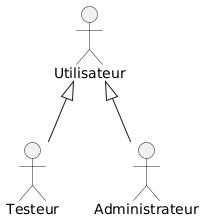
\includegraphics [width=0.5\textwidth]
     {figures/images/Acteurs.png}
    \caption{{Acteurs principales}}
    \label{fig:Acteurs principales}
\end{figure}









\subsection{Diagramme de cas d’utilisation}

Le diagramme de cas d’utilisation illustre les interactions entre les acteurs (utilisateur et admin) et les différentes fonctionnalités du système.


\begin{table}[H]
\centering
\rowcolors{2}{blue!10!white}{white}
\renewcommand{\arraystretch}{1.5}
\begin{tabular}{|>{\bfseries}m{3.5cm}|m{10cm}|}
\hline
\rowcolor{blue!20}
\textbf{Acteur} & \textbf{Fonctionnalités / Actions} \\
\hline
\textbf{Testeur} & 
\begin{itemize}[label=\textbullet]
    \item Authentification via l'interface sécurisée (connexion).
    \item Construction dynamique d'un message ISO 8583 (saisie des champs MTI, champ 2, champ 3, etc.).
    \item Validation d'une transaction ISO 8583 (achat, retrait, consultation de solde, recharge, etc.).
    \item Réception d'une réponse ISO automatiquement générée (MTI 0210 avec le champ 39).
    \item Consultation de l'historique des transactions (filtrage par date, MTI, statut, etc.).
    \item Exportation d'une validation en PDF via JasperReports.
    \item Utilisation des fonctionnalités supplémentaires :
    \begin{itemize}[label=$\triangleright$]
        \item \textbf{Packing} : Convertir un JSON en message ISO.
        \item \textbf{Depacking} : Lire un message ISO et voir ses champs décomposés.
        \item \textbf{Téléchargement} : Télécharger la réponse ou le message décomposé en format \texttt{CSV}, \texttt{XML}, \texttt{JSON}, \texttt{TXT}, \texttt{ISO}.
    \end{itemize}
\end{itemize} \\
\hline
\textbf{Administrateur} & 
\begin{itemize}[label=\textbullet]
    \item Authentification via une interface sécurisée.
    \item Accès à toutes les validations et historiques de tous les utilisateurs.
    \item Suppression totale ou partielle des validations si nécessaire.
    \item Réception de notifications en cas d'anomalies (échecs répétés).
    \item Accès à un tableau de bord de monitoring et de statistiques techniques.
    \item Visualisation des logs centralisés dans le microservice de monitoring.
\end{itemize} \\
\hline
\end{tabular}
\caption{Fonctionnalités par acteur dans le diagramme de cas d'utilisation}
\label{tab:use-case-fonctionnalites}
\end{table}




Le diagramme montre également des relations d'inclusion (<<include>>) et d'extension (<<extend>>), indiquant que certaines actions, comme la consultation des détails d'une entreprise, sont nécessaires pour accéder à des fonctionnalités supplémentaires, telles que le lancement d’un itinéraire. Le diagramme du cas d'utilisation ci-dessous se traduit de cette manière :



\begin{figure}[H]
    \centering
     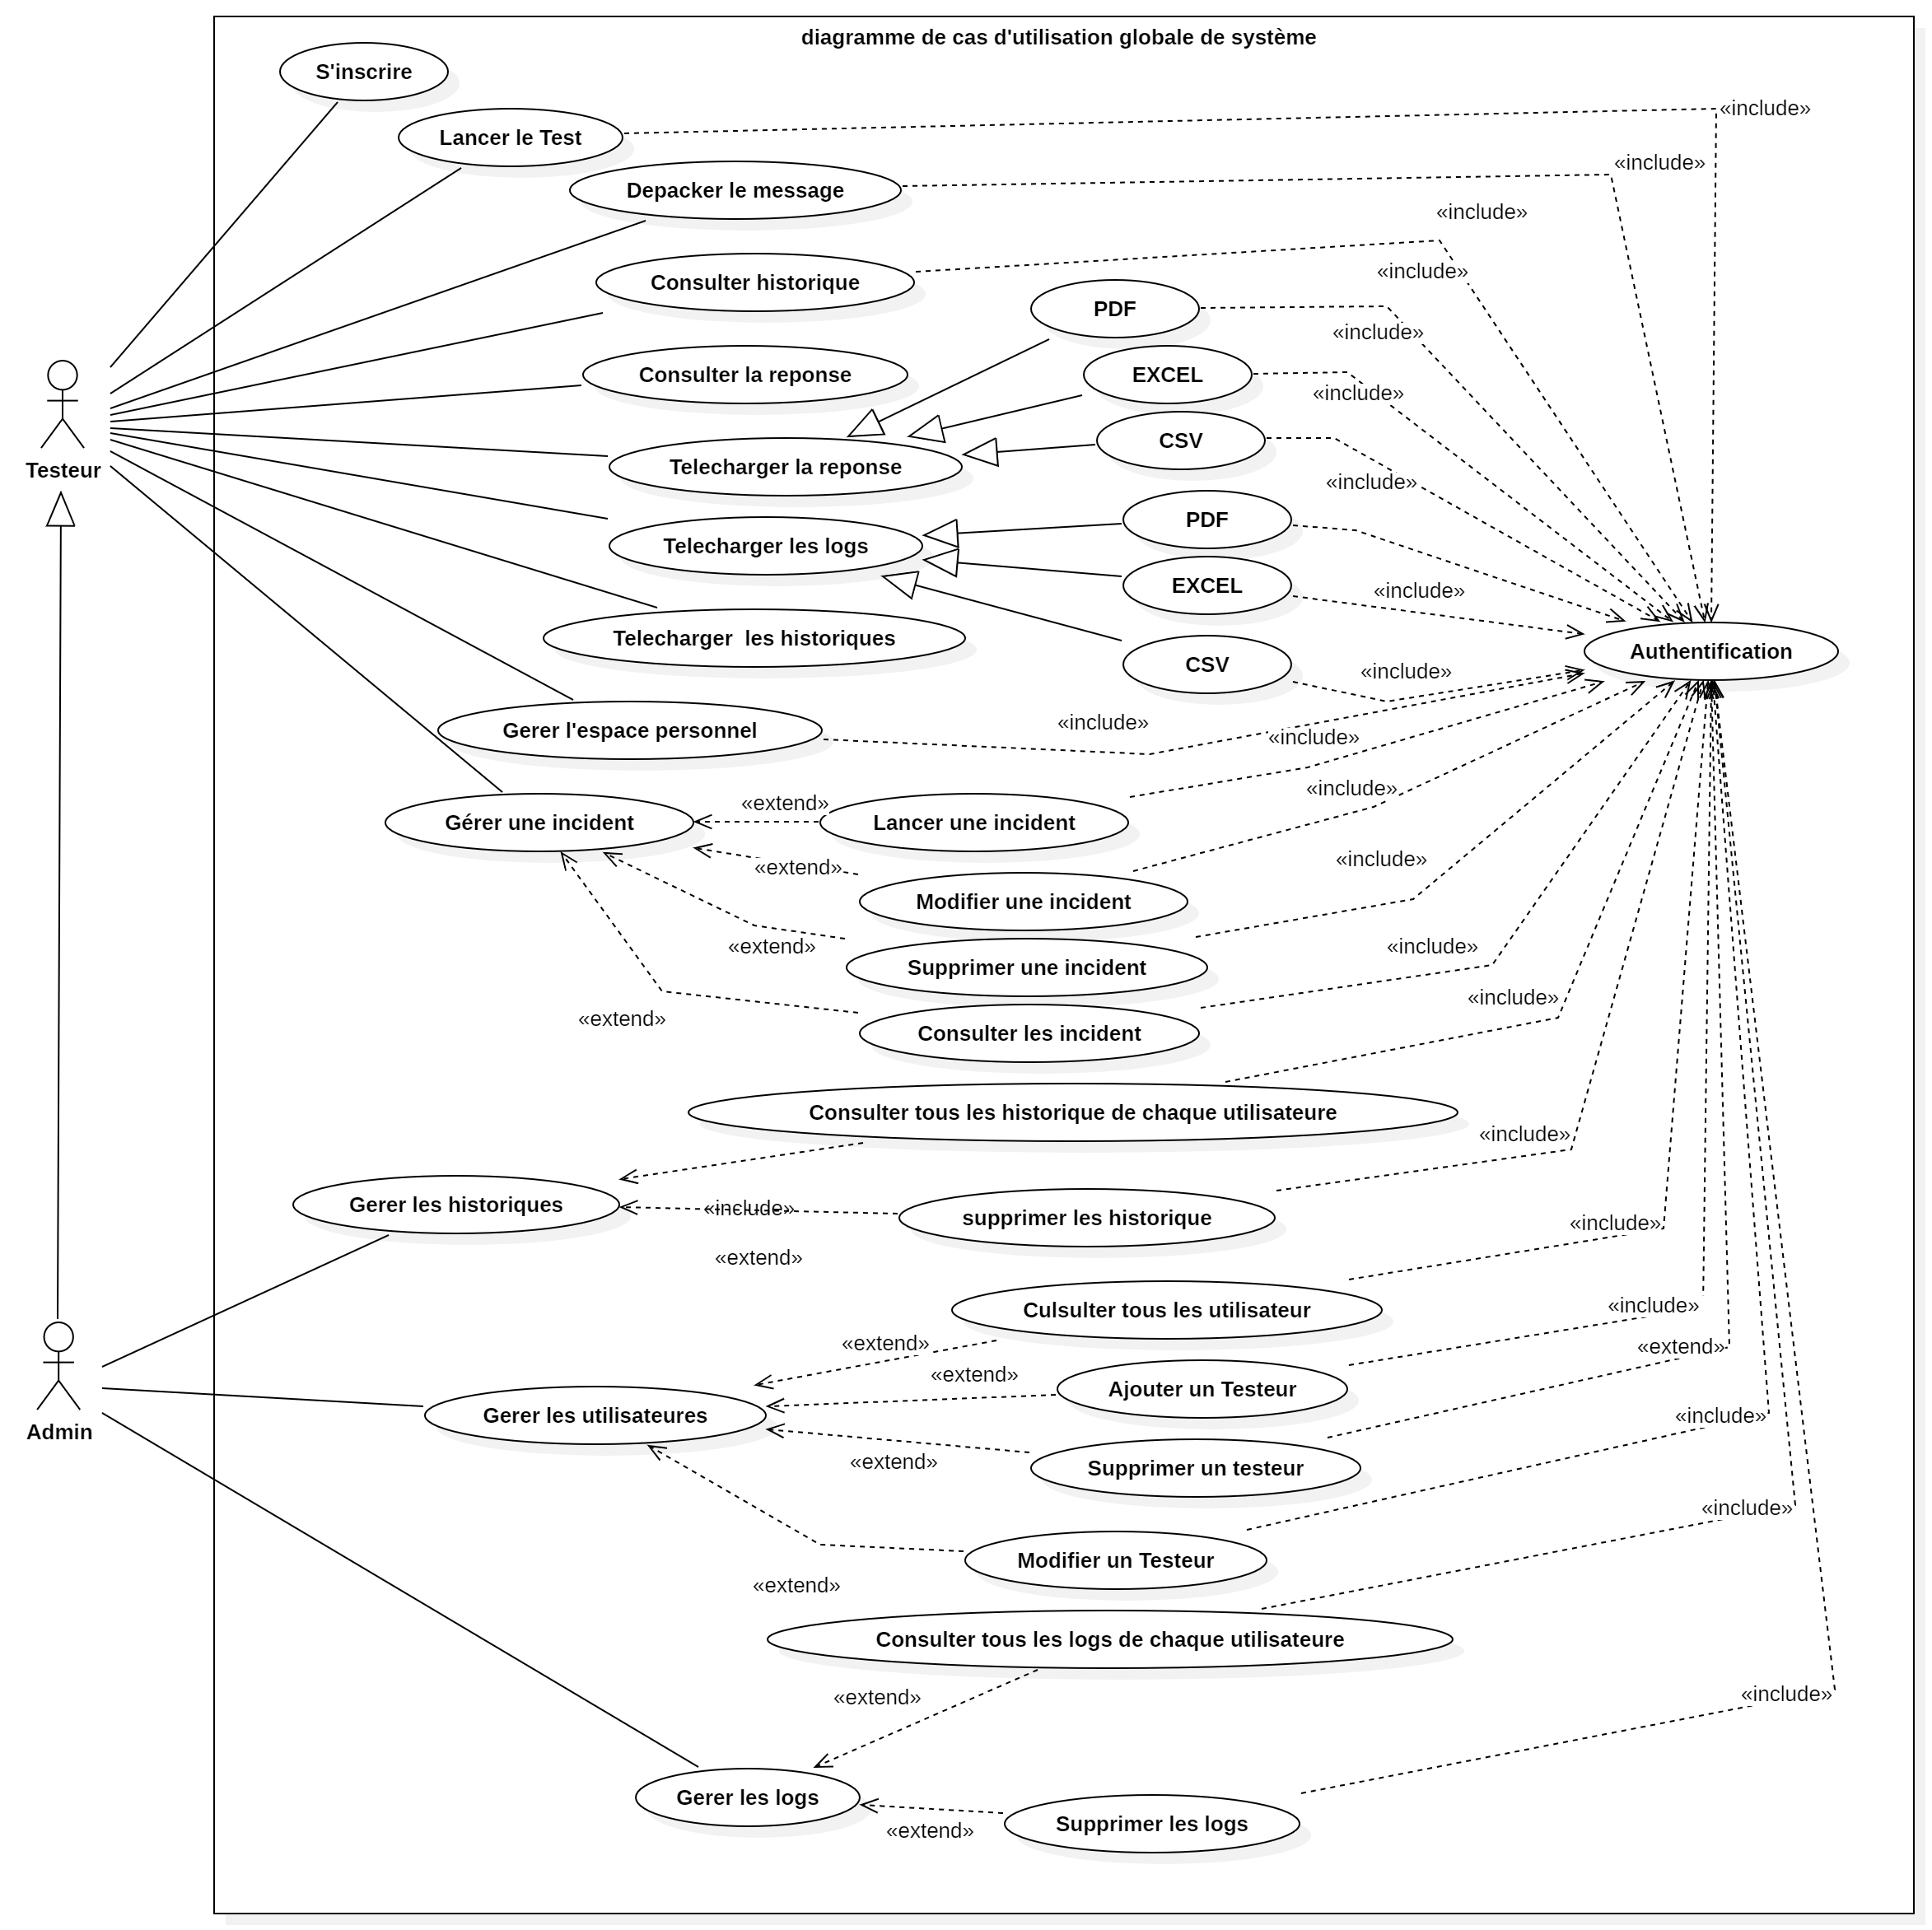
\includegraphics [width=1\textwidth]
     {figures/images/UseCaseDiagramFinal.png}
    \caption{{Diagramme de cas d'utilisation}}
    \label{fig:Diagramme de Gantt}
\end{figure}


\subsection{Diagrammes de séquences}
Un diagramme de séquence est un diagramme UML  qui représente la séquence de messages entre les objets au cours d'une interaction. Un diagramme de séquence comprend un groupe d'objets, représentés par des lignes de vie, et les messages que ces objets échangent lors de l'interaction \cite{uml-omg}.

\subsubsection{Diagramme de séquence de cas d’utilisation « Authentification »}
\addcontentsline{toc}{subsubsection}{{Diagramme de séquence de cas d’utilisation « Authentification »}
Le diagramme présenté ci-dessous illustre le déroulement du cas d’utilisation ”S’authentifier”. Selon ce scénario, le développeur doit entrer le nom d’utilisateur et le mot de passe fourni par l’administrateur. Le développeur doit changer obligatoirement le premier mot de passe. Si ce dernier est changé, alors il est redirigé vers la page d’accueil ; sinon, un message d’erreur s’affiche.

\begin{figure}[H]
    \centering
     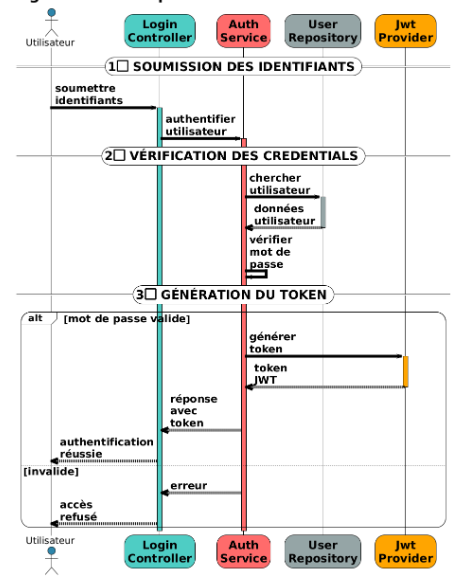
\includegraphics [width=1\textwidth]
     {figures/images/AuthSequence.png}
    \caption{{Diagramme de l'authentification}}
    \label{fig:Diagramme de l'authentification}
\end{figure}

Ce diagramme de séquence illustre le processus d’authentification d’un utilisateur via un système sécurisé utilisant des tokens JWT.

Le processus commence lorsque l’utilisateur soumet ses identifiants via le \texttt{LoginController}. Le contrôleur transmet ensuite la requête au \texttt{AuthService}, qui est chargé d’authentifier l’utilisateur. Le service interroge la base de données via le \texttt{UserRepository} pour rechercher les informations de l’utilisateur.

Une fois les données récupérées, le service vérifie la validité du mot de passe fourni. Deux scénarios peuvent alors se produire :
\begin{itemize}[label=\textbullet]
    \item \textbf{Si le mot de passe est valide :} Le \texttt{JwtProvider} génère un token JWT qui est renvoyé à l’utilisateur via le \texttt{LoginController}, indiquant une authentification réussie.
    \item \textbf{Si le mot de passe est invalide :} Une erreur est renvoyée, et l’accès est refusé.
\end{itemize}

Ce diagramme met en évidence les échanges entre les différentes entités du système (\texttt{LoginController}, \texttt{AuthService}, \texttt{UserRepository} et \texttt{JwtProvider}) et montre la logique conditionnelle qui gère les cas de succès et d’échec d’authentification.


\subsubsection{Diagramme de séquence – Génération et traitement d’un message ISO}
\begin{figure}[H]
\centering
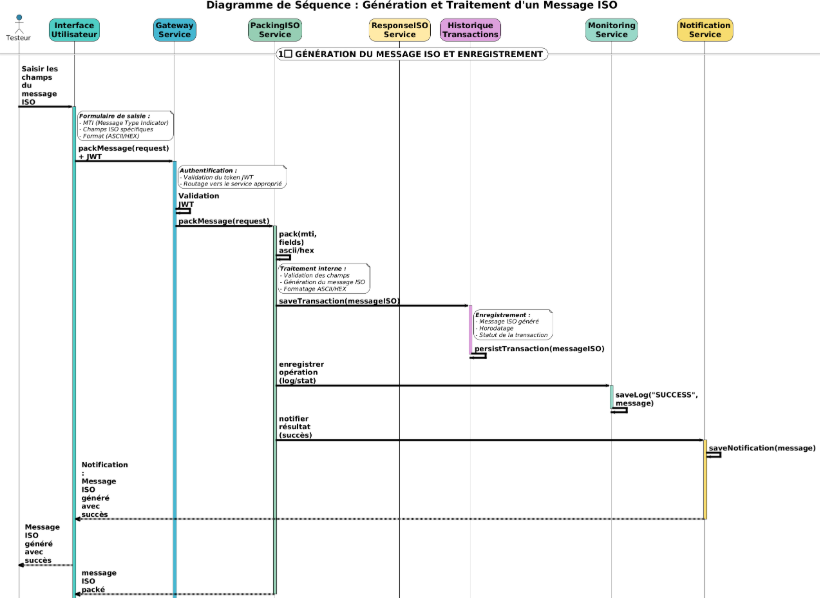
\includegraphics[width=1\textwidth]{figures/images/DS_GenerationMesaage1.PNG}
\caption{Diagramme de séquence – Traitement automatique de la réponse ISO}
\label{fig:mobile_app_architecture}
\end{figure}

\begin{figure}[H]
\centering
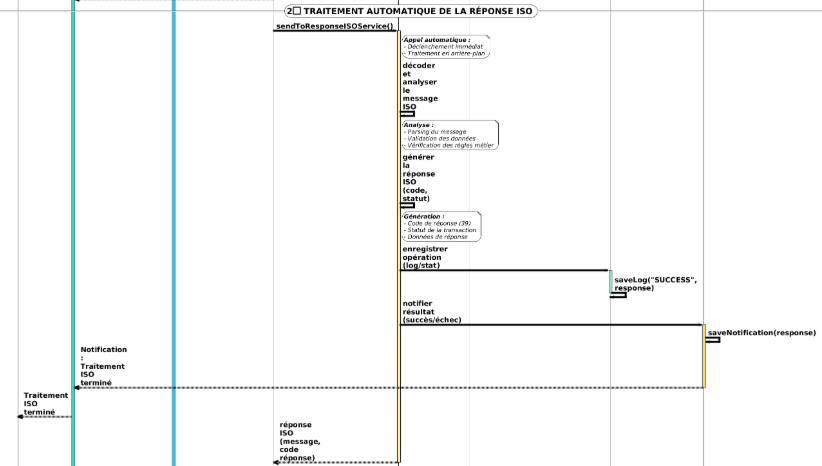
\includegraphics[width=1\textwidth]{figures/images/DS_GenerationMesaage2.png}
\caption{Diagramme de séquence – Affichage du résultat }
\label{fig:mobile_app_architecture}
\end{figure}

\begin{figure}[H]
\centering
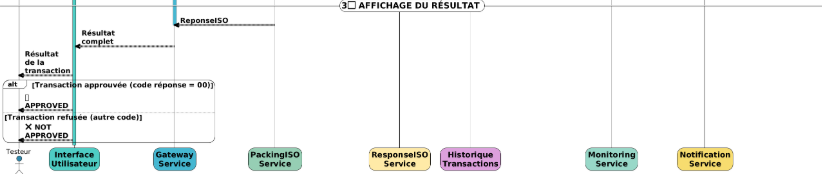
\includegraphics[width=1\textwidth]{figures/images/DS_GenerationMessage3.png}
\caption{Diagramme de séquence – Affichage du résultat}
\label{fig:mobile_app_architecture}
\end{figure}




Le diagramme de séquence illustre l'interaction entre l'utilisateur et le système pour afficher une carte avec des entreprises et leurs zones de chaleur, tout en permettant l'application de filtres spécifiques. Voici les étapes détaillées de ce processus : 

\begin{itemize}[label=$\bullet$]
    \item \textbf{Lancement de l'affichage de la carte avec les entreprises} : L'utilisateur commence par interagir avec l'interface de la carte. Le système répond en chargeant et en affichant une carte contenant les entreprises ainsi que leurs zones de chaleur. Ces zones représentent des indicateurs d'investissement, mettant en évidence les endroits où il est interdit d'investir. 
    \item \textbf{Application de filtres par l'utilisateur} : L'utilisateur peut ensuite appliquer plusieurs types de filtres pour affiner les résultats. Les filtres disponibles incluent la ville, le secteur d'activité, la forme juridique et le nom de l'entreprise. Ces critères permettent de restreindre l'affichage aux entreprises qui correspondent aux préférences de l'utilisateur. 
    \item \textbf{Chargement des entreprises filtrées} : Suite à l'application des filtres, le système traite la demande et recherche à nouveau les entreprises en fonction des filtres définis. Une fois le processus de filtrage terminé, la carte est mise à jour pour afficher uniquement les entreprises correspondantes, accompagnées de leurs zones de chaleur respectives. 
    \item \textbf{Affichage de la carte mise à jour} : Le système renvoie la carte filtrée à l'utilisateur, permettant ainsi une visualisation plus ciblée des entreprises avec les zones à éviter pour les investissements. 
\end{itemize}

\subsubsection{Diagramme de séquence du Dépacking d'un message ISO 8583}
\begin{figure}[H]
\centering
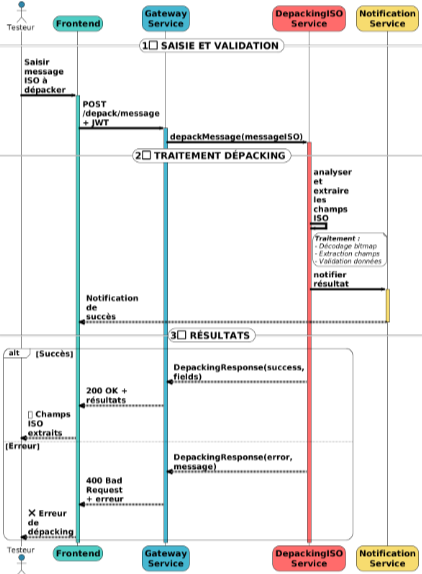
\includegraphics[width=1\textwidth]{figures/images/DS_DepackISO.png}
\caption{ Diagramme de séquence – Dépacking d’un message ISO 8583 }
\label{fig:mobile_app_architecture}
\end{figure}

Ce diagramme de séquence illustre le processus complet de dépacking d’un message ISO 8583 soumis par un utilisateur, ainsi que la gestion des notifications associées.

Il met en évidence les interactions entre les différents composants du système :
\begin{itemize}[label=$\bullet$]
    \item L’utilisateur,
    \item Le \texttt{DepackingController} et le \texttt{DepackingService},
    \item Le composant technique \texttt{ISO8583Packager},
    \item Le \texttt{NotificationService}.
\end{itemize}

\vspace{0.3cm}

\textbf{Déroulement du scénario :}

\begin{itemize}[label=$\bullet$]
    \item \textbf{Soumission du message :} L’utilisateur envoie un message ISO 8583 à dépacker via \textbf{UI}, qui le transmet au \texttt{DepackingController}.
    
    \item \textbf{Traitement du message :} Le contrôleur appelle la méthode \texttt{depackIsoMessage} du \texttt{DepackingService}, qui délègue l’analyse technique du message au composant \texttt{ISO8583Packager} (basé sur la librairie jPOS).
    
    \item \textbf{Analyse et extraction :}
    \begin{itemize}[label=$\triangleright$]
        \item Si le message est valide, les champs sont extraits et structurés.
        \item Si le message est invalide (format incorrect, champs manquants, etc.), une erreur est générée.
    \end{itemize}

    \item \textbf{Gestion des notifications :}
    \begin{itemize}[label=$\triangleright$]
        \item En cas de succès, le \texttt{DepackingService} envoie une notification de succès au \texttt{NotificationService}, qui confirme la réception.
        \item En cas d’échec, une notification d’échec est également envoyée et confirmée.
    \end{itemize}
    
    \item \textbf{Retour à l’utilisateur :}
    \begin{itemize}[label=$\triangleright$]
        \item Si le dépacking est réussi, le contenu structuré est retourné à l’utilisateur.
        \item En cas d’erreur, un message d’erreur explicite est renvoyé.
    \end{itemize}
\end{itemize}


Ce diagramme permet de visualiser clairement :
\begin{itemize}[label=$\bullet$]
    \item La chaîne de traitement du message ISO.
    \item La séparation des responsabilités entre les composants.
    \item La traçabilité offerte par le système de notifications.
\end{itemize}
 

\subsection{Diagramme de classe} 

Afin de rendre la conception bien claire, on a modélisé l’application par le diagramme de classe qui est un schéma utilisé pour présenter les classes et les interfaces des systèmes ainsi que leurs relations. Le diagramme ci-dessous permet de fournir une présentation abstraite des objets du système qui vont interagir ensemble pour réaliser les cas d’utilisation \cite{uml-omg}. 

\begin{figure}[H]
    \centering
     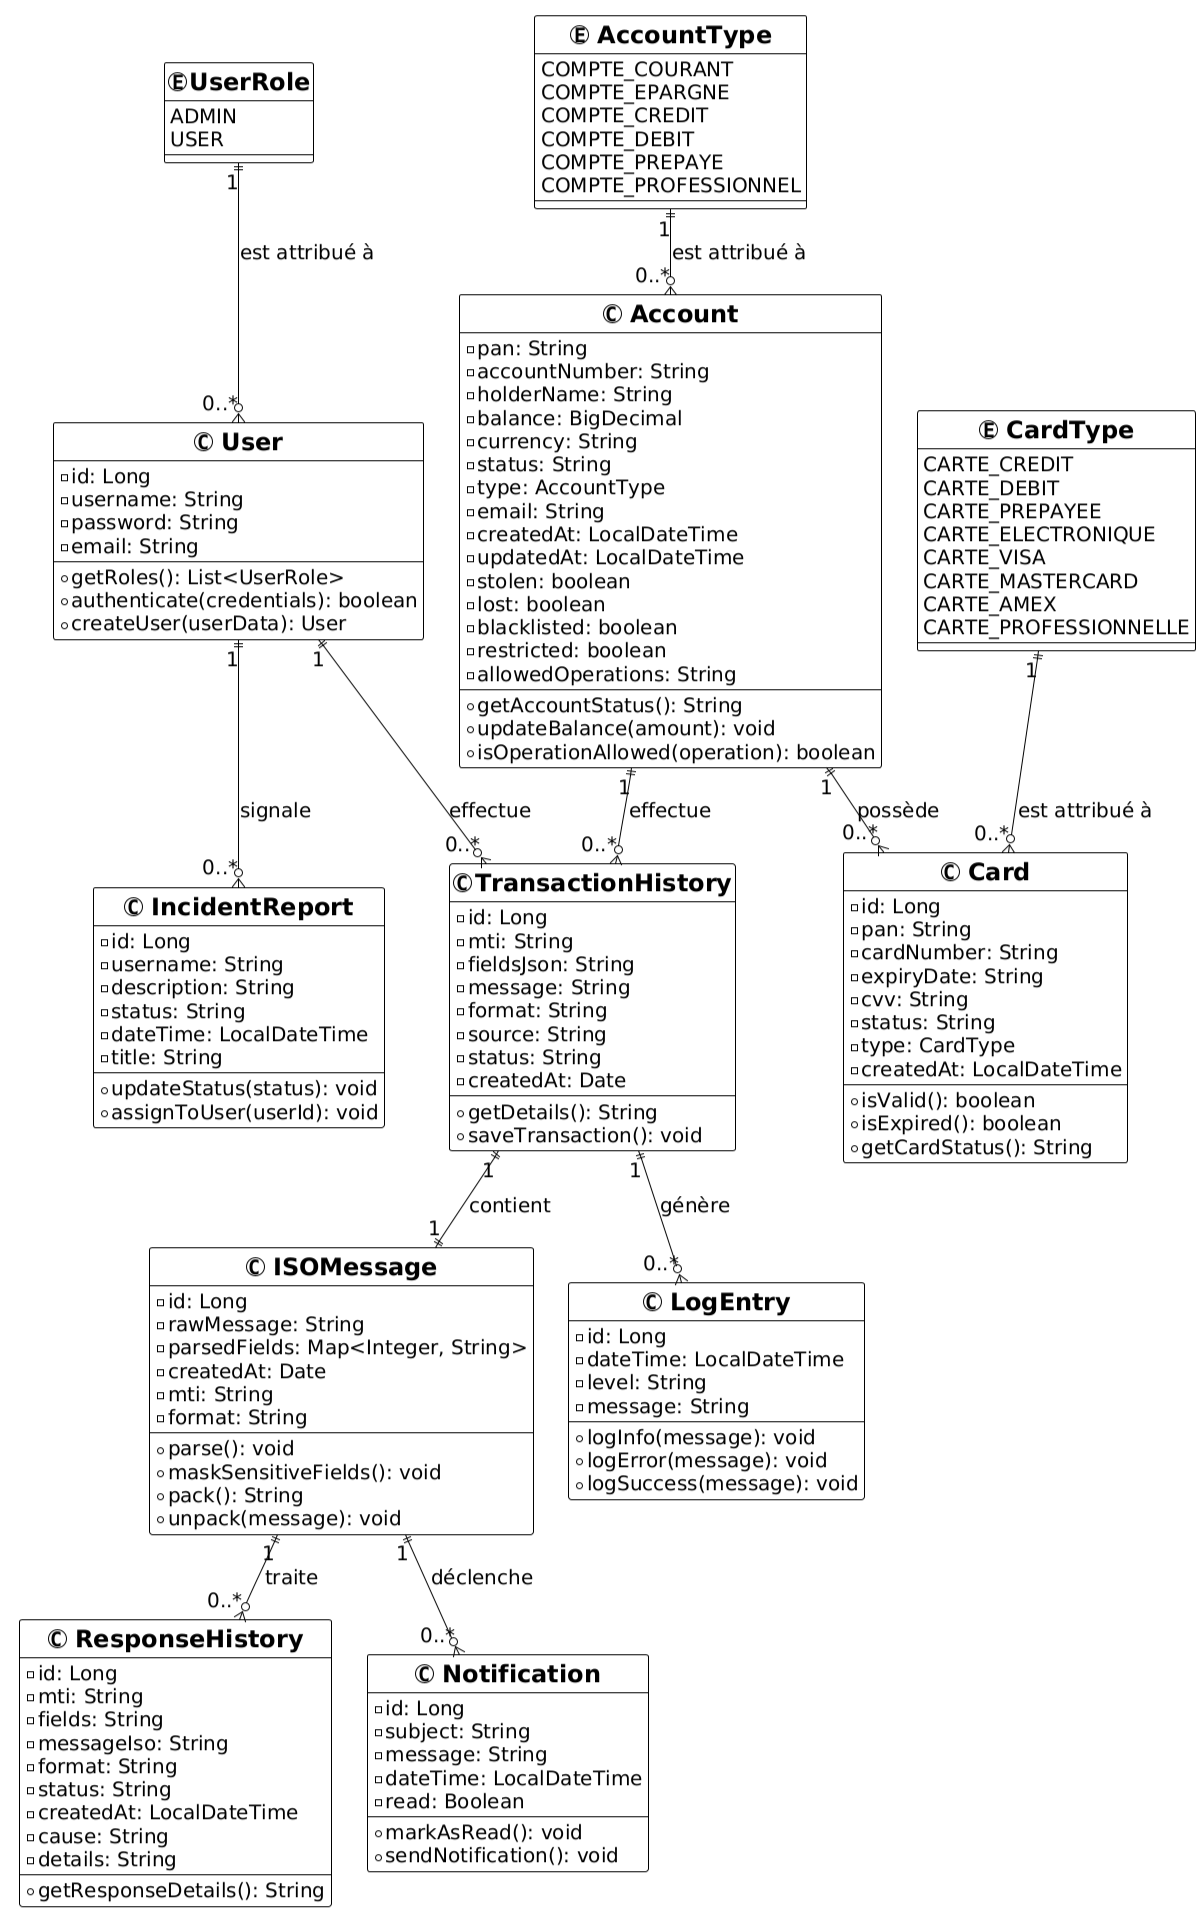
\includegraphics [width=0.9\textwidth]
     {figures/images/DC2.png}
    \caption{{Diagramme de Classe}}
    \label{fig:Diagramme de Classe}
\end{figure}

Ce diagramme présente la structure principale du modèle de données du projet, centré sur la gestion des messages ISO 8583, des utilisateurs, des rôles, des logs, des notifications et de l’historique des transactions.

\begin{table}[H]
\centering
\rowcolors{2}{blue!10!white}{white}
\renewcommand{\arraystretch}{1.5}
\begin{tabular}{|>{\bfseries}m{4cm}|m{11cm}|}
\hline
\rowcolor{blue!20}
\textbf{Classe} & \textbf{Description} \\
\hline
\textbf{User} & Représente un utilisateur du système, possédant un ou plusieurs rôles (UserRole, modélisé ici comme une énumération). \\
\hline
\textbf{UserRole} & Définit les différents rôles possibles pour un utilisateur, tels que ADMIN ou USER. \\
\hline
\textbf{Account} & Représente un compte bancaire associé à un utilisateur, avec des informations sur le solde, la devise, le statut et le type de compte. \\
\hline
\textbf{Card} & Représente une carte de paiement associée à un compte, avec des informations sur le PAN, la date d'expiration et le statut. \\
\hline
\textbf{ISOMessage} & Modélise un message ISO 8583, avec ses champs bruts et extraits, et les méthodes associées pour le parsing et le packing. Cette classe est au cœur du système, car elle est liée à l'historique des transactions, aux logs et aux notifications. \\
\hline
\textbf{TransactionHistory} & Stocke l'historique du traitement des messages ISO, associant chaque transaction à un message ISO et à un type d'opération. \\
\hline
\textbf{IncidentReport} & Représente les incidents signalés par les utilisateurs, avec des informations sur le titre, la description et le statut de résolution. \\
\hline
\textbf{LogEntry} & Permet de tracer les actions effectuées par les utilisateurs. Chaque log est associé à un utilisateur et peut être généré par un message ISO. \\
\hline
\textbf{Notification} & Représente les notifications envoyées aux utilisateurs, en lien avec des actions ou événements sur les messages ISO. \\
\hline
\textbf{ResponseHistory} & Stocke l'historique des réponses aux messages ISO, avec des informations sur le statut, la cause et les détails de la réponse. \\
\hline
\end{tabular}
\caption{Présentation des classes principales du système}
\label{tab:classes-principales}
\end{table}


\subsection*{Relations entre les classes}

Les relations dans ce diagramme incluent des cardinalités importantes à noter :

\begin{itemize}[label=\textbullet]
    \item \textbf{User et UserRole} : Un utilisateur (\texttt{User}) peut avoir un seul rôle (\texttt{UserRole}), ce qui permet de gérer les droits d'accès et les profils dans le système. 
    La relation est de type \texttt{1 à 0..*} (un rôle peut être attribué à plusieurs utilisateurs, mais chaque utilisateur n'a qu'un seul rôle).

       \item \textbf{User et Incident\nobreak Report} : Un utilisateur peut signaler plusieurs incidents (\texttt{Incident\break Report}). Chaque incident est associé à un utilisateur, assurant ainsi la traçabilité des problèmes signalés.

    \item \textbf{User et TransactionHistory} : Un utilisateur peut effectuer plusieurs transactions (\texttt{TransactionHistory}). Chaque transaction est associée à un utilisateur, permettant de suivre l'historique des opérations par utilisateur.

    \item \textbf{Account et Card} : Un compte bancaire (\texttt{Account}) peut posséder plusieurs cartes (\texttt{Card}). Chaque carte est associée à un seul compte, permettant la gestion des moyens de paiement multiples.

    \item \textbf{Account et TransactionHistory} : Un compte bancaire peut être impliqué dans plusieurs transactions (\texttt{TransactionHistory}). Chaque transaction est associée à un compte, assurant le suivi des opérations financières.

        \item \textbf{User et Transaction\nobreak History} : Un utilisateur peut effectuer plusieurs transactions (\texttt{Transaction\break History}). Chaque transaction est associée à un utilisateur, permettant de suivre l'historique des opérations par utilisateur.


    \item \textbf{ISOMessage et ResponseHistory} : Un message ISO peut être traité par plusieurs réponses (\texttt{ResponseHistory}), permettant de gérer les différents états et réponses du message.

    \item \textbf{ISOMessage et Notification} : Un message ISO peut déclencher plusieurs notifications (\texttt{Notification}), par exemple pour informer un utilisateur du succès ou de l'échec d'un traitement.

    \item \textbf{TransactionHistory et LogEntry} : Chaque historique de transaction peut générer plusieurs entrées de log (\texttt{LogEntry}), assurant ainsi la traçabilité complète des opérations.

    \item \textbf{AccountType et Account} : Un type de compte (\texttt{AccountType}) peut être attribué à plusieurs comptes (\texttt{Account}), permettant la catégorisation des comptes bancaires.

    \item \textbf{CardType et Card} : Un type de carte (\texttt{CardType}) peut être attribué à plusieurs cartes (\texttt{Card}), permettant la catégorisation des moyens de paiement.
\end{itemize}

\subsection{Diagramme d'activité}

Un diagramme d'activité UML est un type de diagramme comportemental qui modélise le flux de travail ou le processus métier d'un système. Il décrit les activités, les décisions, les conditions et les flux de contrôle entre les différentes étapes d'un processus, permettant ainsi de visualiser et de comprendre le déroulement logique des opérations \cite{uml-omg}.


\begin{figure}[H]
\centering
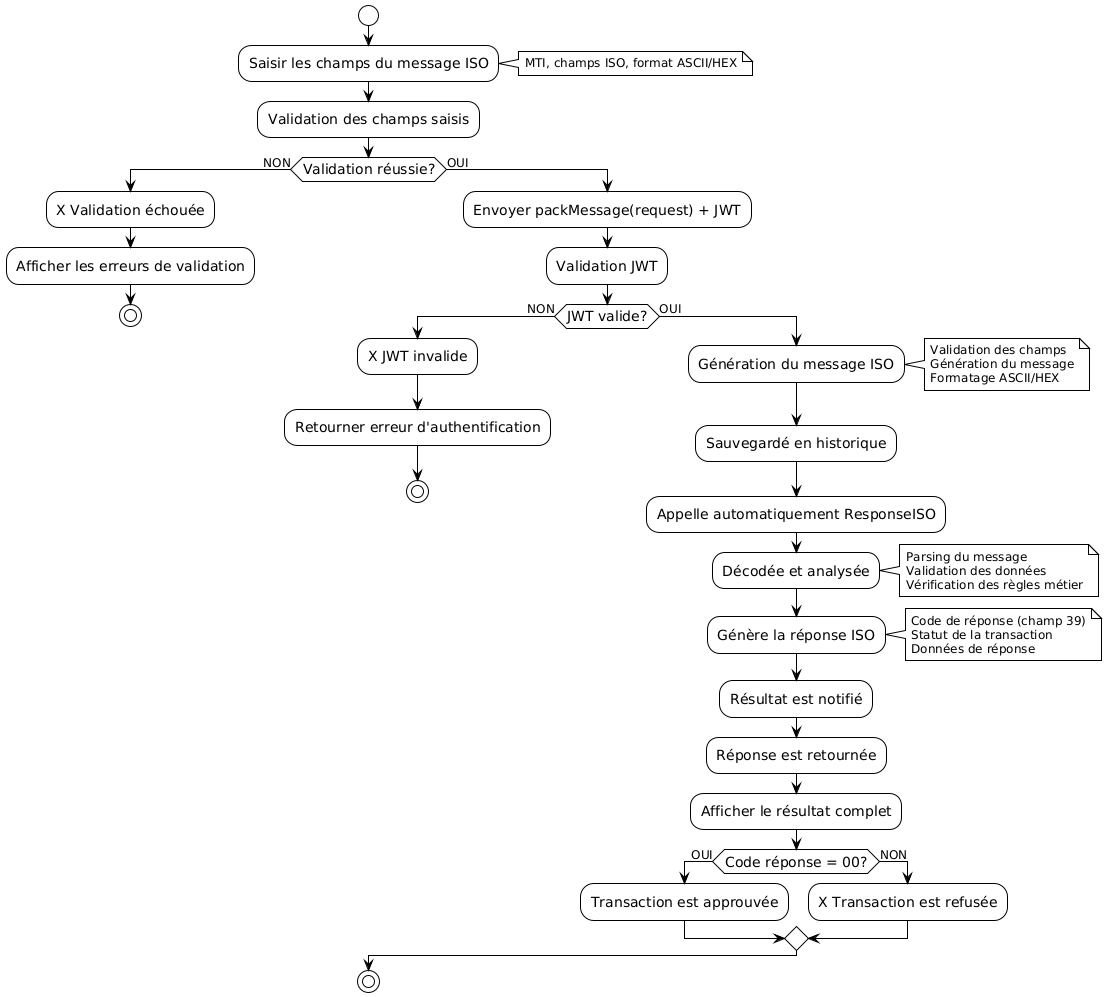
\includegraphics[width=0.8\textwidth]{figures/images/DA_generationMessage2.png}
\caption{Diagramme d'activité de la génération et du traitement d'un message ISO}
\label{fig:diagramme-activite-iso}
\end{figure}
Ce diagramme d'activité illustre le flux complet de la génération et du traitement d'un message ISO au sein du simulateur HPS. Il décrit les étapes séquentielles, les décisions et les chemins alternatifs, depuis la saisie initiale des champs jusqu'à l'affichage du résultat final de la transaction.

Le processus débute par l'activité de saisie des champs du message ISO, où l'utilisateur renseigne les informations nécessaires via un formulaire incluant le MTI (Message Type Indicator), des champs ISO spécifiques et le format (ASCII/HEX). Le système procède ensuite à la validation des champs saisis, avec gestion des erreurs de validation en cas d'échec.

Si la validation est réussie, le système effectue une authentification JWT avant de procéder à la génération du message ISO. Le message généré est sauvegardé en historique et le système appelle automatiquement le service ResponseISO pour simuler la réponse. Cette réponse est décodée, analysée et traitée pour générer une réponse ISO appropriée.

Le processus se termine par l'affichage du résultat complet, avec une gestion différenciée selon le code de réponse : approbation de la transaction en cas de succès (code 00) ou affichage des erreurs et actions correctives en cas d'échec.


\section*{Conclusion}

Ce chapitre a permis de clarifier les spécifications essentielles du projet, tant sur le plan fonctionnel que technique. Les différentes fonctionnalités attendues ont été présentées, ainsi que les choix architecturaux, justifiés en fonction des besoins du système. Cette analyse constitue une base solide pour l'exposé de l'architecture technique globale du projet, ainsi que pour la phase de conception détaillée et la mise en œuvre effective du simulateur. Le chapitre suivant sera dédié à la présentation des technologies utilisées, à la description de l'environnement de développement et à l'exposition de l'architecture microservices du projet.



